\documentclass[12pt]{article}

\usepackage{sbc-template}

\usepackage{graphicx,url}
\usepackage{pdflscape}


%\usepackage[brazil]{babel}   
\usepackage[utf8]{inputenc}  
\usepackage{float}

     
\sloppy

\title{Classificação de \textit{fake news} utilizando Aprendizado de Máquina}

\author{Murilo Luis C. Neves\inst{1}, Vitor Padovani\inst{1}, Fernando Silva Grande\inst{1}}


\address{Departamento de Informática -- Universidade Estadual de Maringá}

\begin{document} 

\maketitle

\begin{abstract}
  This meta-paper describes the style to be used in articles and short papers
  for SBC conferences. For papers in English, you should add just an abstract
  while for the papers in Portuguese, we also ask for an abstract in
  Portuguese (``resumo''). In both cases, abstracts should not have more than
  10 lines and must be in the first page of the paper.
\end{abstract}
     
\begin{resumo} 
  Este meta-artigo descreve o estilo a ser usado na confecção de artigos e
  resumos de artigos para publicação nos anais das conferências organizadas
  pela SBC. É solicitada a escrita de resumo e abstract apenas para os artigos
  escritos em português. Artigos em inglês deverão apresentar apenas abstract.
  Nos dois casos, o autor deve tomar cuidado para que o resumo (e o abstract)
  não ultrapassem 10 linhas cada, sendo que ambos devem estar na primeira
  página do artigo.
\end{resumo}

\section{Introdução}

Falar um pouco sobre fake news e aprendizado de máquina...

\section{Fundamentação Teórica}

\subsubsection{Random Forest}

\subsubsection{Logistic Regression}

\subsubsection{Gradient Boosting}

\subsubsection{Redes Neurais}

\section{Materiais e métodos}

	Nesta seção, são descritos os materiais utilizados para o trabalho (seção \ref{sec:materiais}) e os métodos como foram trabalhados (seção \ref{sec:metodos}).
	
\subsection{Materiais} \label{sec:materiais}

Os materiais utilizados para esse trabalho incluem o \textit{dataset} WELFake, e, como ferramentas de codificação principais, as bibliotecas \textit{Scikit-Learn}, \textit{Spacy} e \textit{Torch}.

\subsubsection{Base de dados}

O \textit{dataset} utilizado é o WELFake, devido ao grande volume de dados presentes no mesmo e um relativo balanceamento entre as classes real e falso. Ele possui 72134 entradas, onde 35028 são reais e 37106 são falsas. No entanto, como é mostrado na seção \ref{sec:preproc}, há duplicatas, o que torna o número de entradas válidas no \textit{dataset} menor.

O \textit{dataset} possui como colunas o identificador de cada texto, título, texto e \textit{label}, onde a \textit{label} 0 indica notícia falsa e 1 indica notícia real. Um ponto importante de ser notado é que, como o \textit{dataset} não possui \textit{features} pré-extraídas (apenas possui o texto em si), elas foram posteriormente extraídas pelos discentes (seção \ref{sec:preproc}).

Uma análise inicial indica a seguinte proporção de duplicatas:

\begin{table}[h]
	\centering
	\begin{tabular}{|l|c|}
		\hline
		Duplicatas em títulos & 9786 \\
		Duplicatas em textos & 9415 \\
		Duplicatas em linhas inteiras & 8456 \\
		\hline
	\end{tabular}
	\label{tab:duplicatas}
	\caption{Quantidade de duplicatas encontradas na base de dados}
\end{table}

Para este trabalho, considerou-se que apenas duplicatas tanto em título quanto em textos deveriam ser removidas. Alguns gráficos que mostram a distribuição dos tamanhos dos textos e títulos seguem.

\begin{figure}[h]
	\centering
	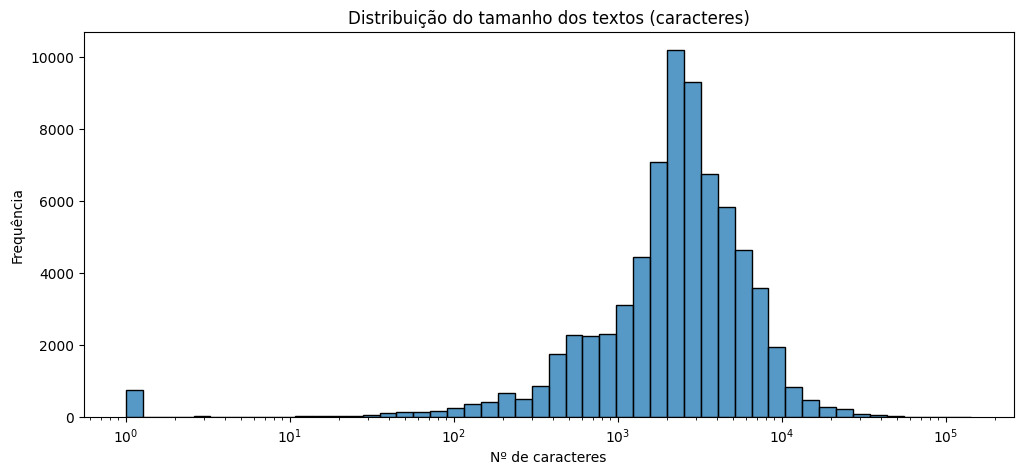
\includegraphics[width=0.6\linewidth]{imagens/preproc/tamanho_textos_char.png}
	\caption{Distribuição dos tamanhos dos textos (em caracteres)}
	\label{fig:preproc_tam_txt_char}
\end{figure}


\begin{figure}[h]
	\centering
	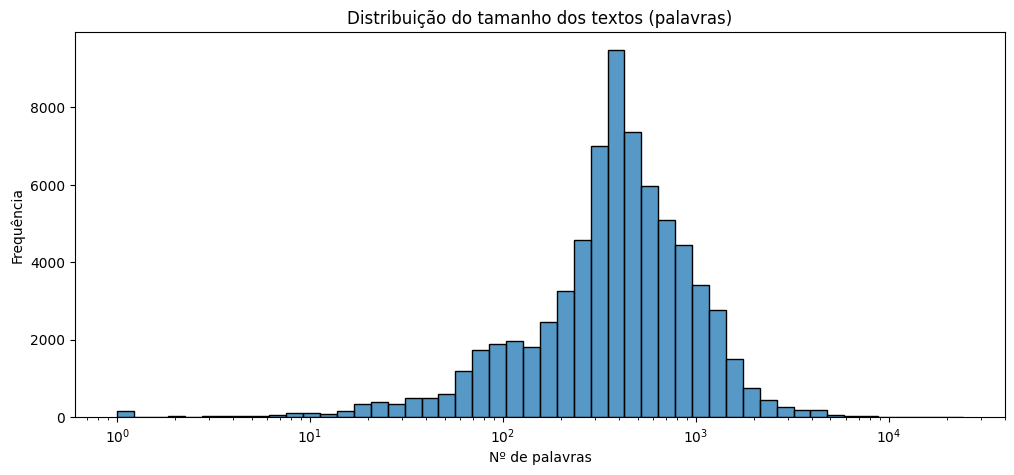
\includegraphics[width=0.6\linewidth]{imagens/preproc/tamanho_textos_palavras.png}
	\caption{Distribuição dos tamanhos dos textos (em palavras)}
	\label{fig:preproc_tam_txt_pal}
\end{figure}


\begin{figure}[h]
	\centering
	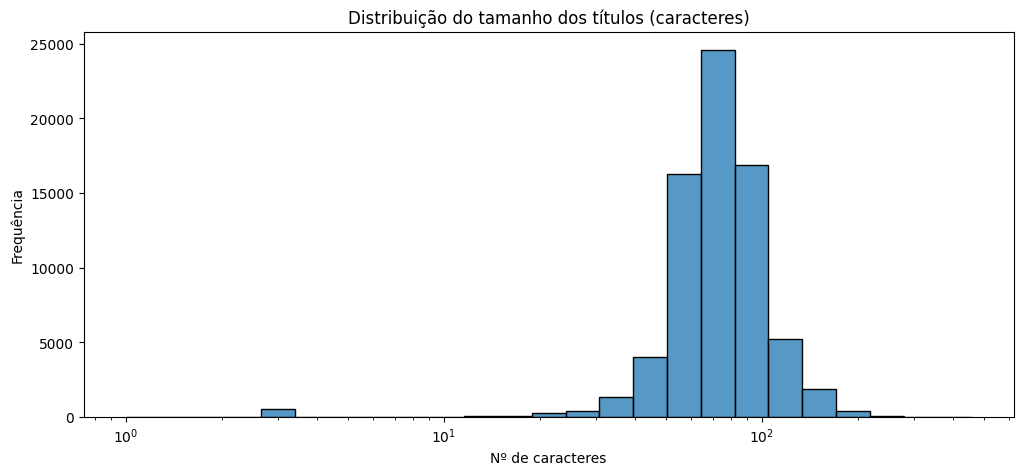
\includegraphics[width=0.6\linewidth]{imagens/preproc/tamanho_titulos_chars.png}
	\caption{Distribuição dos tamanhos dos títulos (em caracteres)}
	\label{fig:preproc_tam_tit_char}
\end{figure}

\subsubsection{Scikit-Learn}

\subsubsection{Spacy}

\subsubsection{Torch}

\subsection{Métodos} \label{sec:metodos}

Nesta seção são descritos os métodos utilizados. Por curiosidade, foram explorados dois métodos de se trabalhar com os dados, nomeados 1 e 2, além de haver um pré-processamento necessário (seção \ref{sec:preproc}).

\subsubsection{Pré-processamento} \label{sec:preproc}

Nesta etapa, um primeiro passo importante é a retirada das duplicatas, a fim de evitar possíveis \textit{data leaks} para os modelos. Além disso, como haviam entradas onde uma das colunas (ora texto, ora título) era nula, foi considerado como 'texto' das entradas a concatenação de título e texto, separados por um espaço.

Após isso, para que fosse possível a execução do método 1, foi-se necessário definir \textit{features} a serem extraídas dos textos para que, a partir delas, fosse criado um novo \textit{dataset} apenas com as \textit{features extraídas}. Para tanto, foram definidas as \textit{features} dispostas na tabela a seguir.

\begin{table}[H]
	\centering
	\begin{tabular}{|l|}
	\hline
		Polaridade \\
		Subjetividade \\
		Tamanho médio de palavra  \\
		Tamanho médio de sentença \\
		Número de exclamações \\
		Proporção de \textit{stopwords} \\
		Diversidade léxica \\
		Quantidade de números presentes no texto \\
		Quantidade de entidades nomeadas \\
		Tamanho da maior entidade nomeada \\
		Proporção de pronomes \\
		Número de links \\
		Proporção de adjetivos  \\
		Proporção de advérbios \\
		Proporção de verbos de dúvida/incerteza \\
		Proporção de citações \\
		Pontuação não terminal por sentença \\
		Proporção de \textit{hedges} \\
		Proporção de conjunções coordenativas \\
	\hline
	\end{tabular}
	\label{tab:features}
	\caption{\textit{Features} extraídas dos textos}
\end{table}

Além disso, para o método 2, foram utilizadas como \textit{features} uma composição entre um vetor da frequência TF-IDF (com limite de 5000) e um vetor com os \textit{embeddings} gerados pelo processamento do texto por meio do BERT (MiniLM-L12-V2), que possui 768 dimensões. O tamanho total do vetor de entrada é de 5768 dimensões. No entanto, como não há maneira significativa e intuitiva de se visualizar esse vetor, não foram realizadas visualizações nessa abordagem.

\subsubsection{Método 1: Técnicas clássicas}

Nesse método, foi-se trabalhado com os indicadores extraídos dos textos conjuntamente a alguns algoritmos classificadores da biblioteca \textit{scikit-learn}. Em um primeiro momento, foram definidos os algoritmos a serem testados e os parâmetros para \textit{GridSearch}.

\begin{table}[H]
	\centering
	\begin{tabular}{|l|l|l|}
		\hline
		Algoritmo & Parâmetro & Valores testados \\
		\hline
		Regressão Logística & C & 0.1, 1, 10  \\
		Regressão Logística & Penalidade & l1, l2 \\ 
		Regressão Logística & \textit{Solver} & liblinear \\ 
		\hline
		\textit{Random Forest} & Num. estimadores & 50, 100 \\
		\textit{Random Forest} & \textit{Max. depth} & 5, 10, None \\
		\hline
		\textit{Gradient boosting} & Num. estimadores & 50, 100\\
		\textit{Gradient boosting} & Taxa de aprendizado & 0.1, 0.05\\
		\textit{Gradient boosting} & \textit{Max. depth} & 3, 5\\
		\hline
	\end{tabular}
	\label{tab:gridsearch}
	\caption{Parâmetros explorados durante o \textit{GridSearch}}
\end{table}

Após isso, os modelos foram ranqueados e escolhido o melhor deles. Para este, foi montada a matriz de confusão e feita uma análise de quais \textit{features} foram mais relevantes bem como uma curva de aprendizado para observar possível \textit{overfitting}.

\subsubsection{Método 2: Redes neurais}

Para esse método, foi-se utilizada uma rede neural com duas camas escondidas, a primeira com 512 dimensões e a segunda com 128. O diagrama que ilustra essa rede está a seguir. A taxa de aprendizado foi de 0.0001.

\begin{figure}[h]
	\centering
	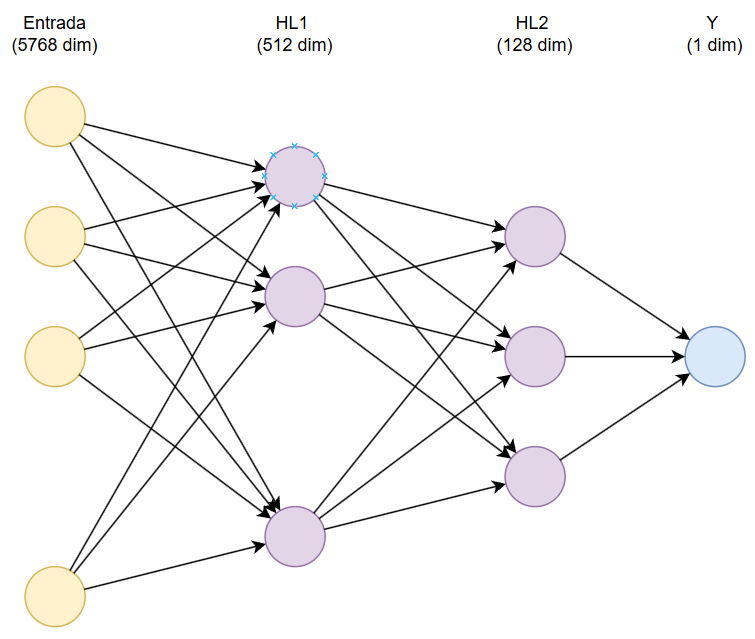
\includegraphics[width=0.6\linewidth]{imagens/rede_neural.png}
	\caption{Rede neural utilizada}
	\label{fig:rede-neural}
\end{figure}

O treino foi configurado com um limite de épocas como sendo 10, mas com um contador de paciência de 5, i.e, após 5 épocas sem melhora no F1-Score, o treino para para evitar \textit{overfitting}.

\section{Resultados}

\subsection{Método 1}

\subsection{Método 2}

O treino no método 2 foi interrompido na nona época devido ao contador de paciência ter se esgotado, e o melhor resultado obtido foi também na nona época. Testes subsequentes com mais épocas e mais flexibilidade no contador não melhoraram significativamente o resultado.

\begin{table}[H]
	\centering
	\begin{tabular}{|l|l|l|l|l|}
		\hline
		Acurácia & Precisão & Recall & F1 & AUC \\
		\hline
		0.9711  & 0.9686 & 0.9676 & 0.9681 & 0.9962 \\
		\hline
	\end{tabular}
	\label{tab:resultados_m2}
	\caption{Resultados obtidos com o método 2}
\end{table}

\pagebreak
\begin{landscape}
\begin{figure}[H]
	\centering
	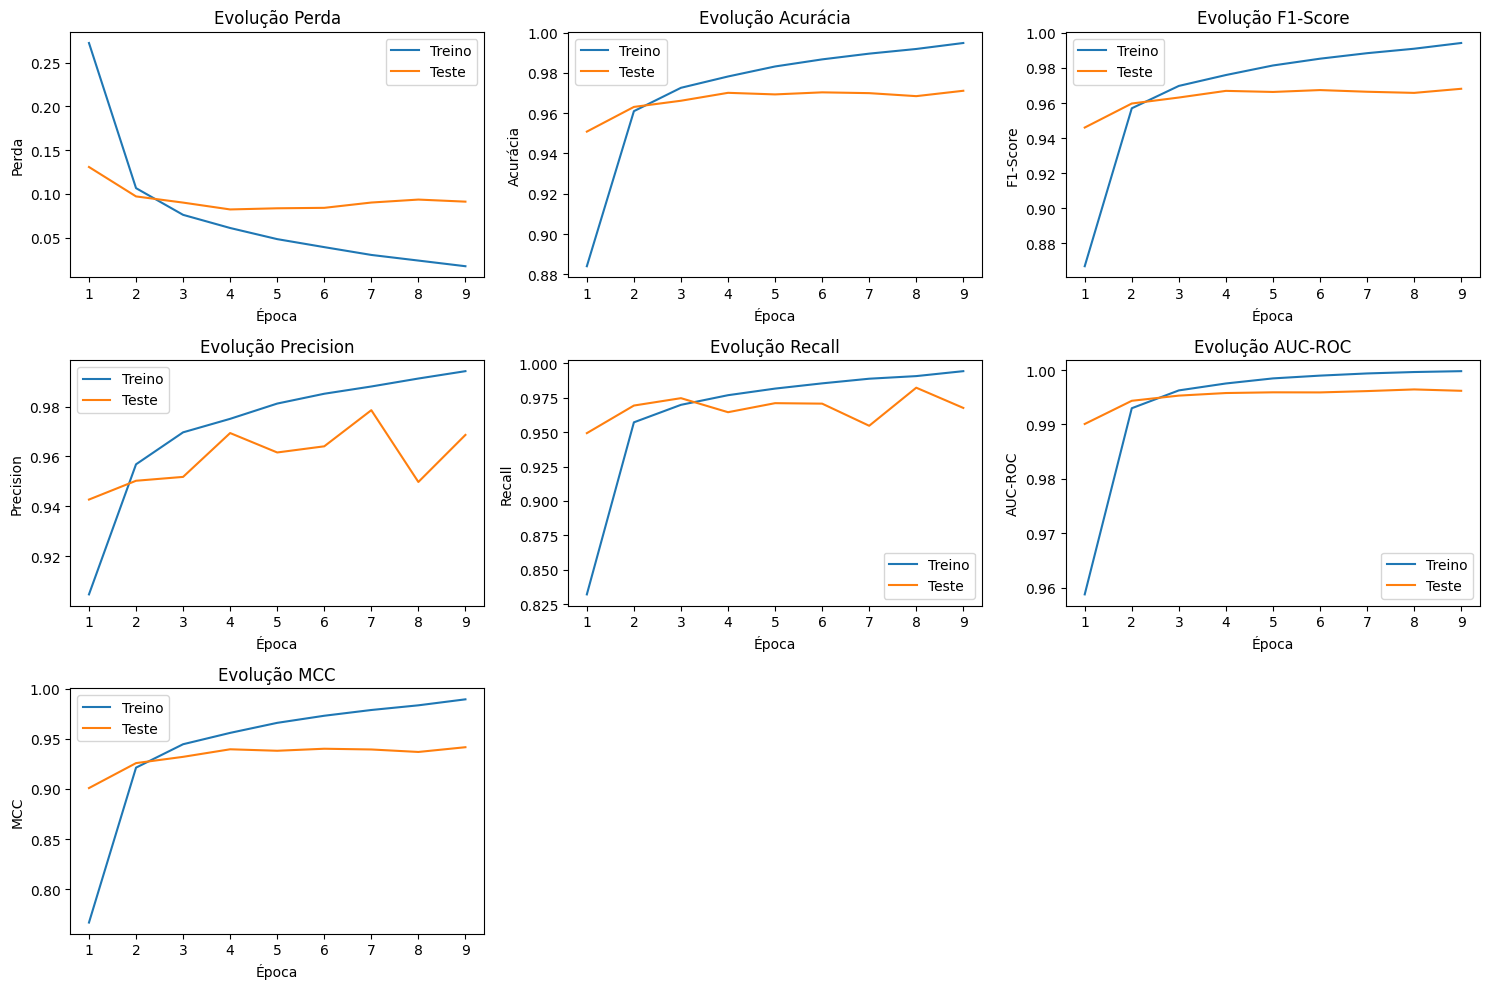
\includegraphics[width=0.85\linewidth]{imagens/resultados_metodo_2.png}
	\caption{Resultados obtidos com o método 2 durante o treinamento}
	\label{fig:resultados_m2}
\end{figure}
\end{landscape}

\section{Conclusões}

\bibliographystyle{sbc}
\bibliography{sbc-template}

\end{document}
